\section{Software Architecture Design}

\subsection{Component Overview}

\begin{table}[h]
\centering
\begin{tabular}{@{}lll@{}}
\toprule
\textbf{Component} & \textbf{Port} & \textbf{Responsibility} \\
\midrule
poll-service & 3000 & Owns the \texttt{polls} collection. Create, list,
    read, and close polls. \\
vote-service & 3001 & Owns the \texttt{votes} collection. Validate and
    record votes. \\
results-service & 3002 & Stateless read model. Aggregates data from
    poll-service and vote-service. \\
notification-service & 3003 & In memory log of poll closed events. No
    persistent storage. \\
mongo & 27017 & Shared database, backing poll-service and vote-service. \\
\bottomrule
\end{tabular}
\caption{Microservices and their responsibilities}
\end{table}

\subsection{Interaction Diagram}

\begin{figure}[h]
\centering
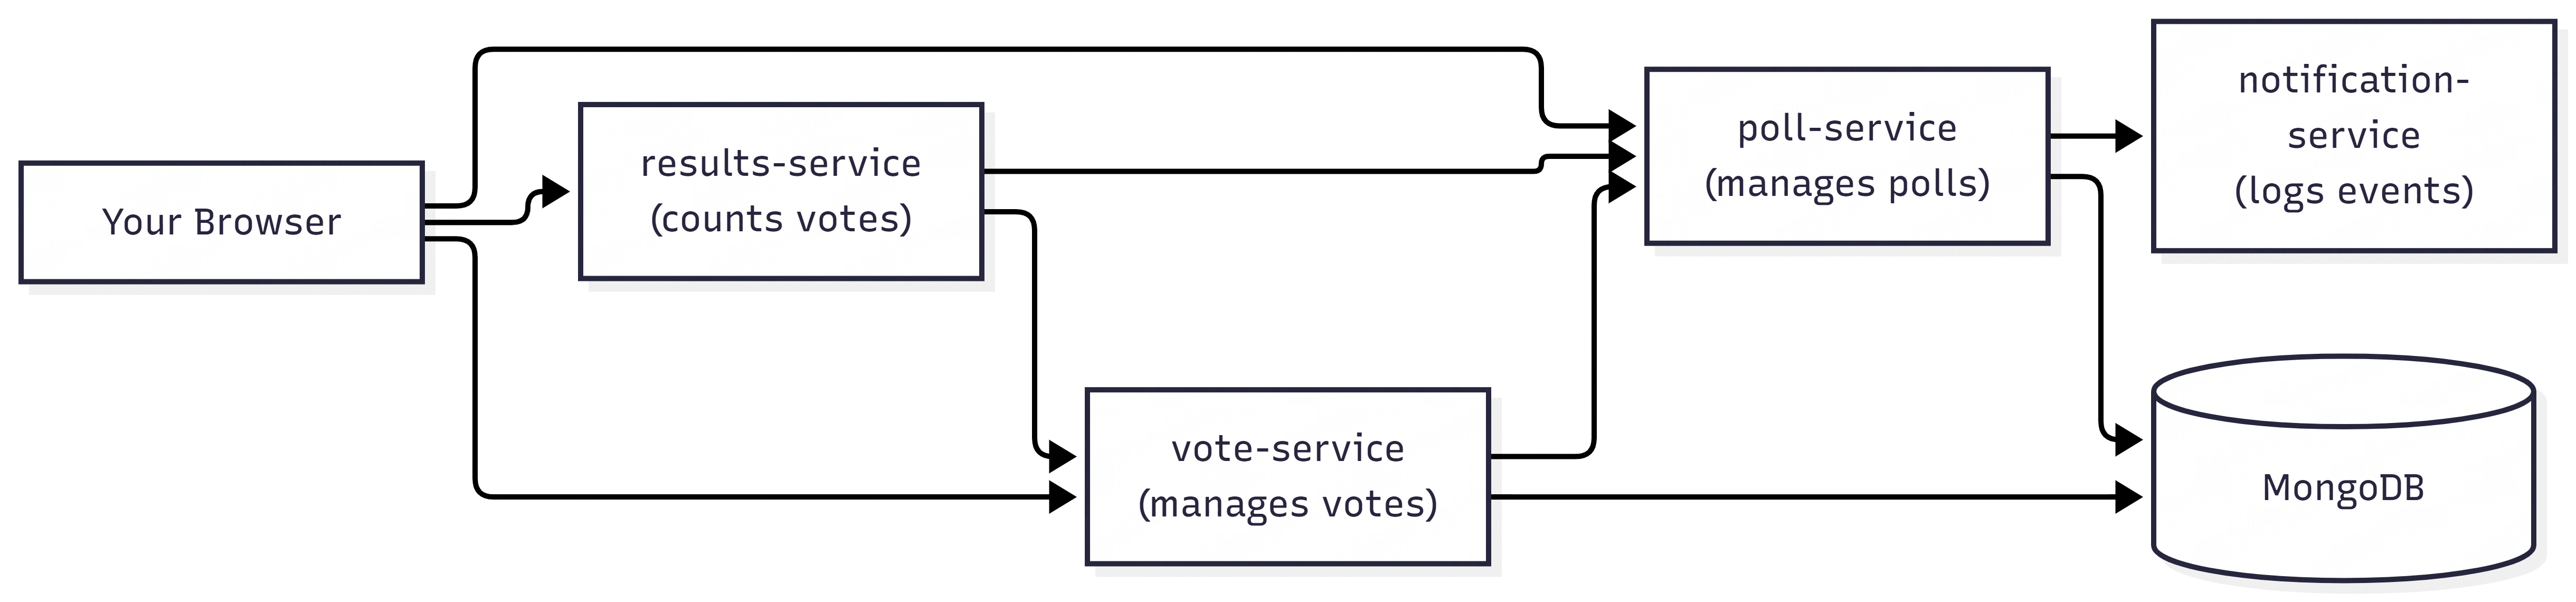
\includegraphics[width=0.9\textwidth]{placeholder.png}
\caption{Interaction between the four microservices and the database}
\end{figure}

Each line in the above diagram is simply an HTTP REST API call. Neither shared memory nor message queues are used; also, there's no access to the database directly from service to service. Poll-service is the only service that both reads and writes the polls database, while vote-service is the only service that both reads and writes the votes database. The results-service doesn't hold any of its own data; rather, it generates data for each of its requests by invoking poll-service and vote-service.

\subsection{Component to Microservice Mapping}

\begin{table}[h]
\centering
\begin{tabular}{@{}ll@{}}
\toprule
\textbf{Conceptual Component} & \textbf{Implementing Microservice} \\
\midrule
Poll management (create, list, read, close) & poll-service \\
Vote casting and duplicate vote prevention & vote-service \\
Live result computation & results-service \\
Poll closed notifications & notification-service \\
Persistent poll and vote storage & mongo (MongoDB) \\
\bottomrule
\end{tabular}
\caption{Mapping from application concepts to deployed microservices}
\end{table}

\subsection{Cloud Architecture Patterns Applied}

\begin{description}[leftmargin=0cm,style=nextline]
    \item[Horizontally Scaling Compute Pattern] results-service is completely stateless and read-only. It does not store any data across requests, and therefore an unlimited number of replicas could be serving traffic simultaneously without any synchronization. That is the part of the application that is designed for scaling-out most.


    \item[Colocate Pattern] All applications and the database work on the same Kubernetes cluster and communicate within the cluster's network, thus maintaining a low latency for collaborating applications.

    \item[Separation of Concerns between provisioning and orchestration]
       Dockerfiles for each individual service exist; however, their job is limited to the creation of the execution environment only. The orchestration (replication, networking, storage), on the other hand, is managed entirely through Kubernetes manifests, and not through Dockerfiles and the application code itself.

    \item[Avoidance of the Queue Centric Workflow Pattern]Purposefully, the app does not have a message queue between the two services. A poll closing notification is pushed directly by using a synchronous REST API call to the notification service without going through the message queue. There was a purpose for that: It is a very simple, one-sided operation, which doesn't require any kind of persistence through possible restarts of the client; therefore, the use of a message queue adds nothing but operational overhead.
\end{description}
